\section{Lecture 7: Parallel Processing}
\subsubsection{Why Parallel Processing?}
\subsubsection{Parallel Computer}
\subsubsection{Parallel Program}
\todo{Allt det här känns som repetition, borde jag skippa?}

\subsection{Architecture classification}
\subsubsection{Flynn’s Classification of Architectures}
\begin{itemize}
\item Single instruction, single data stream - \textbf{SISD} \\
\item Single instruction, multiple data stream - \textbf{SIMD} \\
\item Multiple instruction, single data stream - \textbf{MISD} \\
\item Multiple instruction, multiple data stream- \textbf{MIMD} \\
\end{itemize}

\subsubsection{SISD}
The regular computers who use a single processor, a single instruction stream, and stores data in a single memory.
\subsubsection{SIMD}
Computers with multiple processing elements that perform the same operation on multiple data points simultaneously. There are simultaneous (parallel) computations, but only a single process (instruction) at a given moment.

Array and vector processors are the most common examples of SIMD machines.
\subsubsection{MISD}
Computers where many functional units perform different operations on the same data.
\begin{figure}[H]
  \centering
  \scalebox{0.6}{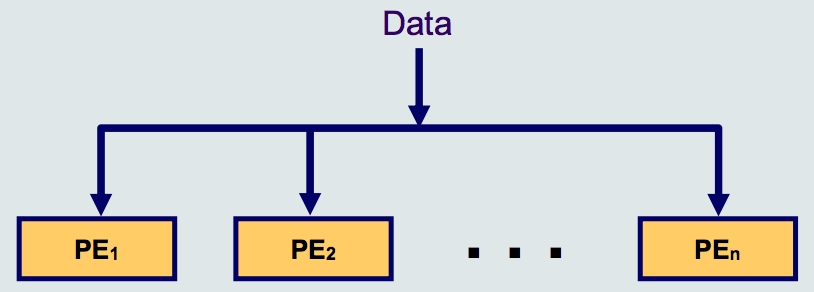
\includegraphics{img/MISD.png}}
  \caption{MISD architecture}
  \label{fig:MISD}
\end{figure}

\subsubsection{MIMD}
A set of processors that simultaneously perform different instructions sequences, on different sets of data.

There is also different classes of MIMD computers:
\begin{itemize}
  \item Shared memory (tightly coupled).
  \begin{itemize}
  \item Symmetric multiprocessor (SMP).
  \item Non-uniform memory access (NUMA).
  \end{itemize}
  \item Distributed memory (loosely coupled) = Clusters.
\end{itemize}

\begin{figure}[H]
  \centering
  \scalebox{0.6}{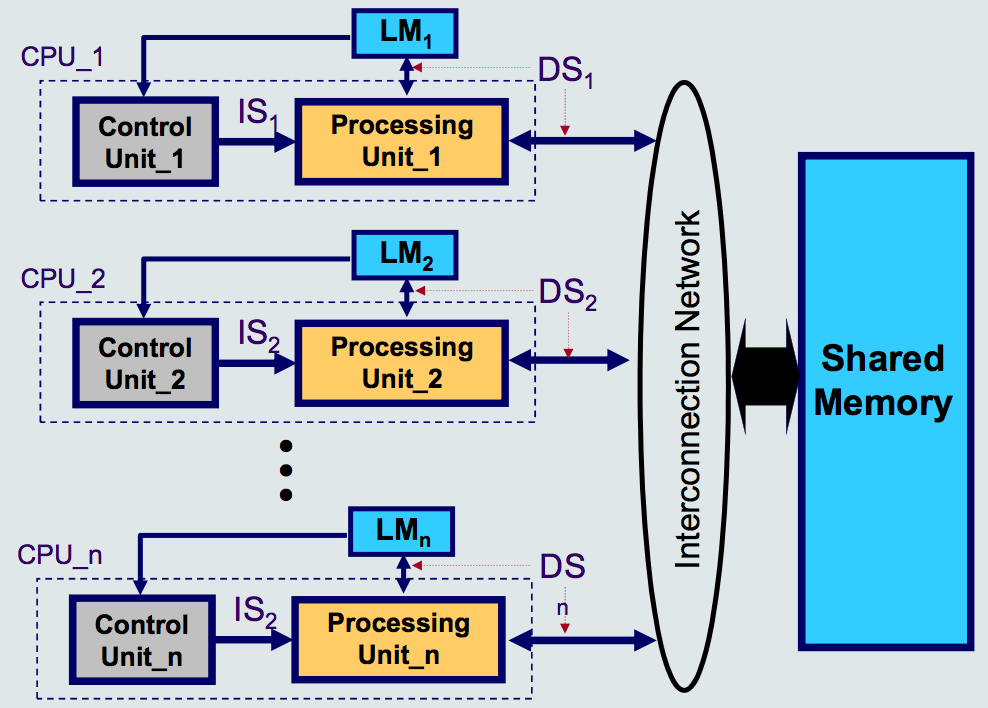
\includegraphics{img/MIMD.png}}
  \caption{MIMD architecture}
  \label{fig:MIMD}
\end{figure}

\subsection{Performance evaluation}
The peak rate of a computer is the maximum value that the computer can work at, this is something that vendors use to sell computers and not something that is really useful for us.

\textbf{Speedup}: measures the gain we get by using a parallel computer, over a sequential one, to run a given application

$$S = \frac{T_s}{T_p}$$

$T_s$ : execution time needed with the sequential computer. \\
$T_p$ : execution time needed with the parallel computer. \\

\textbf{Efficiency}: to relate speedup to the number of processors used, it provides therefore a measure of the efficiency with which the processors are used.

$$E = \frac{S}{P}$$

$S$: speedup. \\
$P$: number of processors. \\
For the ideal situation, in theory: $S = P$; which means $E = 1$.

\textbf{Practically the ideal efficiency of 1 cannot be achieved!}

\subsubsection{Amdahls Law}
Gives the theoretical speedup in latency of the execution of a task at fixed workload that can be expected of a system whose resources are improved.

$$S_{latency}(s)=\frac{1}{1-p+\frac{p}{s}}$$

where
\begin{itemize}
\item $S_{latency}$ is the theoretical speedup in latency of the execution of the whole task;
\item $s$ is the speedup in latency of the execution of the part of the task that benefits from the improvement of the resources of the system;
\item $p$ is the percentage of the execution time of the whole task concerning the part that benefits from the improvement of the resources of the system before the improvement.
  \newline
\end{itemize}

Furthermore:
\begin{equation*}
  \begin{cases}
    S_{latency}(s) \leq \frac{1}{1-p} \\
    \lim_{s \to \infty} = \frac{1}{1-p}
  \end{cases}
\end{equation*}

show that the theoretical speedup of the execution of the whole task increases with the improvement of the resources of the system and that regardless the magnitude of the improvement, the theoretical speedup is always limited by the part of the task that cannot benefit from the improvement.

Amdahl's law is often used in parallel computing to predict the theoretical speedup when using multiple processors. For example, if a program needs 20 hours using a single processor core, and a particular part of the program which takes one hour to execute cannot be parallelized, while the remaining 19 hours (p = 0.95) of execution time can be parallelized, then regardless of how many processors are devoted to a parallelized execution of this program, the minimum execution time cannot be less than that critical one hour. Hence, the theoretical speedup is limited to at most 20 times (1/(1 -- p) = 20). For this reason parallel computing is relevant only for a low number of processors and very parallelizable programs. This can be seen in figure \ref{fig:amdahls-law}

\begin{figure}[H]
  \centering
  \scalebox{0.6}{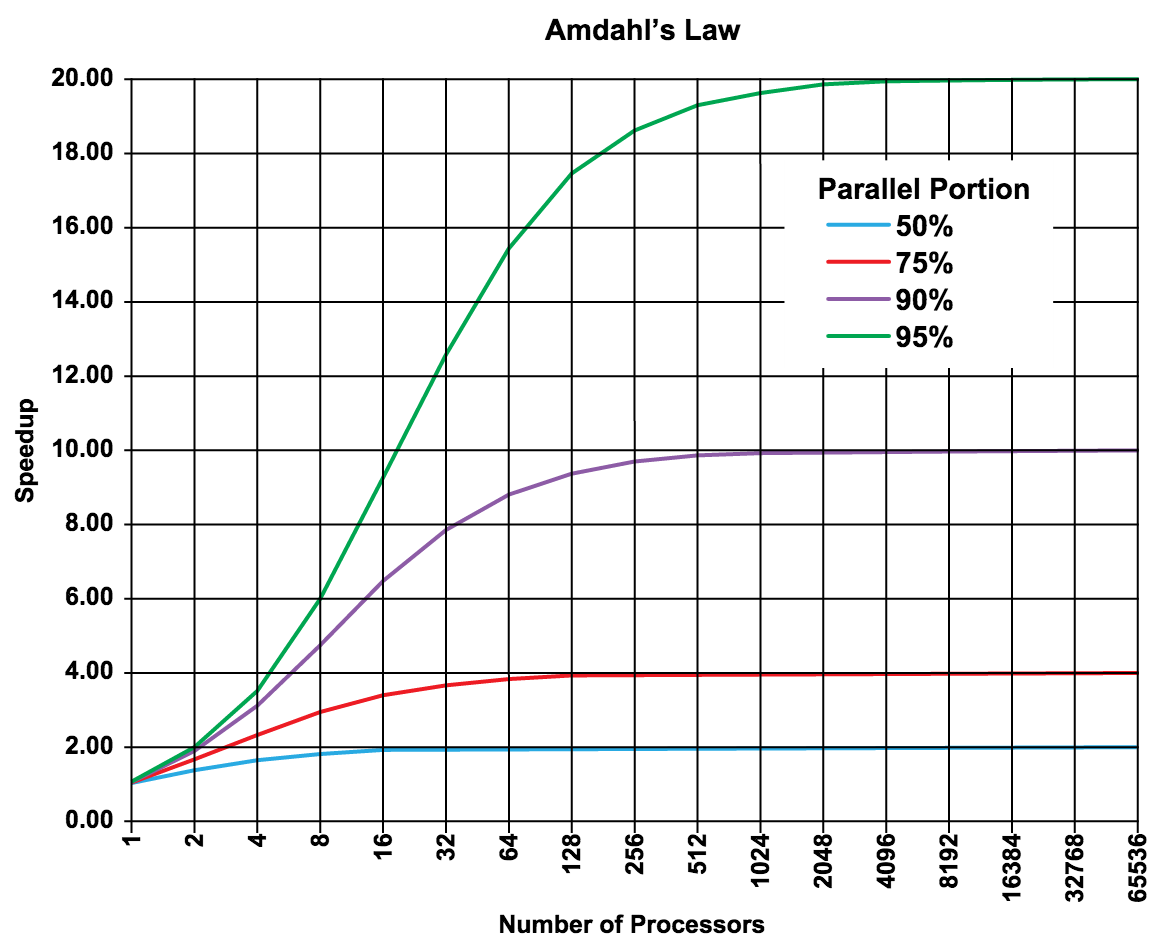
\includegraphics{img/amdahls-law.png}}
  \caption{Amdahls Law}
  \label{fig:amdahls-law}
\end{figure}

\todo{skipped other factors that limit speedup} \\
\todo{and impact of communications}

\subsection{Interconnection network}
Interconnecting Networks (IN) is a key component of parallel computers and has a decisive influence on
\begin{itemize}
\item overall performance
\item total cost of the architecture
\end{itemize}

The traffic in an IN consists of:
\begin{itemize}
\item data transfer
\item transfer of commands and requests (control information).
\end{itemize}

The key parameters of an IN are:
\begin{itemize}
\item total bandwidth: transferred bits/second.
\item implementation cost. 
\end{itemize}

\subsubsection{Single Bus}
These are simple cheap and relatively flexible. Only one communication is allowed at one time, which means the bandwidth is shared by all nodes.

Its performance is relatively poor, in order to get a good performance the number of nodes needs to be limited (16-20), and we can use several buses instead.
\subsubsection{Completely Connected Network}
Here every is connected to each other, which means that communication can be performed in parallel between any pair of nodes. Performance is high but also the construction cost, which will increase rapidly by every added node.
\subsubsection{Crossbar Network}
A dynamic network: the interconnection topology can be modified by configurating the switches. It is completely connected: any node can be directly connected to any other
\\\todo{borde det inte stå att: kan vara completely connected?}
\subsubsection{Mesh Network}
\begin{itemize}
\item Cheaper than completely connected networks, while giving relatively good performance.
\item In order to transmit data between two nodes, routing through intermediate nodes is needed (maximum 2(n-1) intermediates for an $n^2$ mesh).
\item It is possible to provide wrap-around connections: Torus.
\item Three dimensional meshes have also been implemented.
\end{itemize}

\begin{figure}
  \hfill
  \subfigure[Regular mesh network]{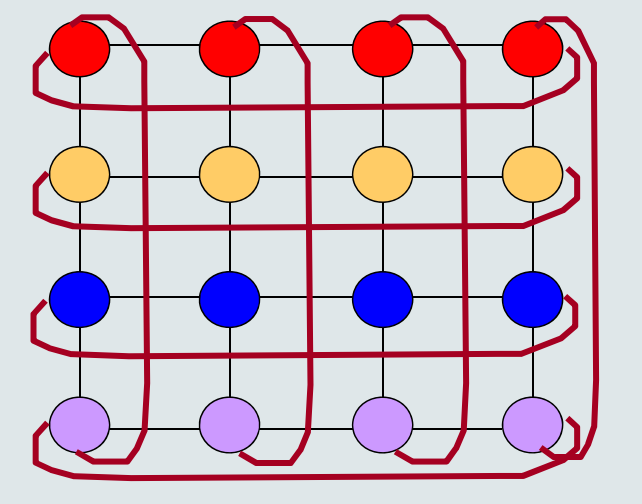
\includegraphics[width=5cm]{img/mesh.png}}
  \hfill
  \subfigure[Torus network]{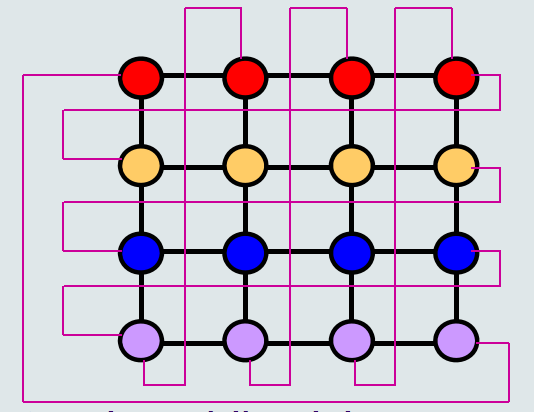
\includegraphics[width=5cm]{img/torus.png}}
  \hfill
  \caption{Mesh Network}
\end{figure}

\subsubsection{Hypercube Network}
$2^n$ nodes are arranged in an n-dimensional cube. Each node is connected to n neighbors.
\begin{figure}[H]
  \centering
  \scalebox{0.6}{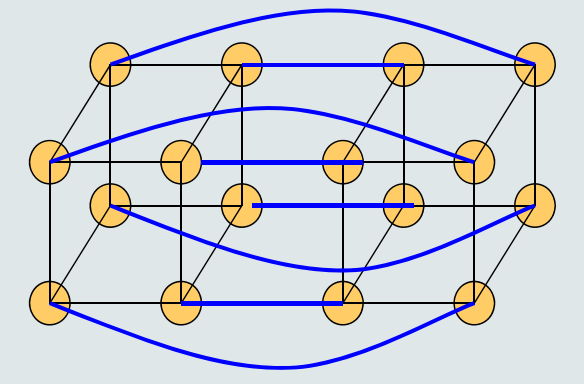
\includegraphics{img/hypercube.png}}
  \caption{Hypercube Network}
  \label{fig:hypercube-network}
\end{figure}
